% Provenance (never printed): old seconde/premiere S material on the
% atmosphere (water vapour, saturation, cloud formation, the vertical motion
% of air) and enseignement scientifique premiere (water cycle); see
% sources/book2/PROVENANCE.md. Every saturation value, lapse rate,
% condensation level and the lee-wind example are computed in
% figdata/grade-10/clouds.py from the IAPWS saturation curves; the soundings
% are invented examples, said so in the text.
\chapter{Por que as nuvens se formam}\label{ch:g10:why-clouds-form}

Num terraço, no verão, um copo de água gelada está sobre a mesa. Em um
minuto, a parte de fora dele se cobre de gotinhas, e um anel de água se
espalha ao seu pé. A água não vazou através do vidro: ela saiu do ar, que
se resfriou onde tocava o copo frio. Algumas horas mais tarde, a
quilômetros acima da planície, a mesma coisa acontece em grande escala:
bolhas de ar quente sobem, se resfriam e, a certa altura, a água que elas
carregam aparece na forma dos montes brancos de base achatada chamados
cúmulos. Este capítulo explica quanto vapor de água o ar pode conter, por
que o ar que sobe se resfria, a que altura as nuvens se formam, por que em
certos dias elas ficam achatadas e em outros se elevam em trovoadas, e
como as minúsculas gotículas de nuvem se transformam em chuva e neve.

\begin{omfigure}
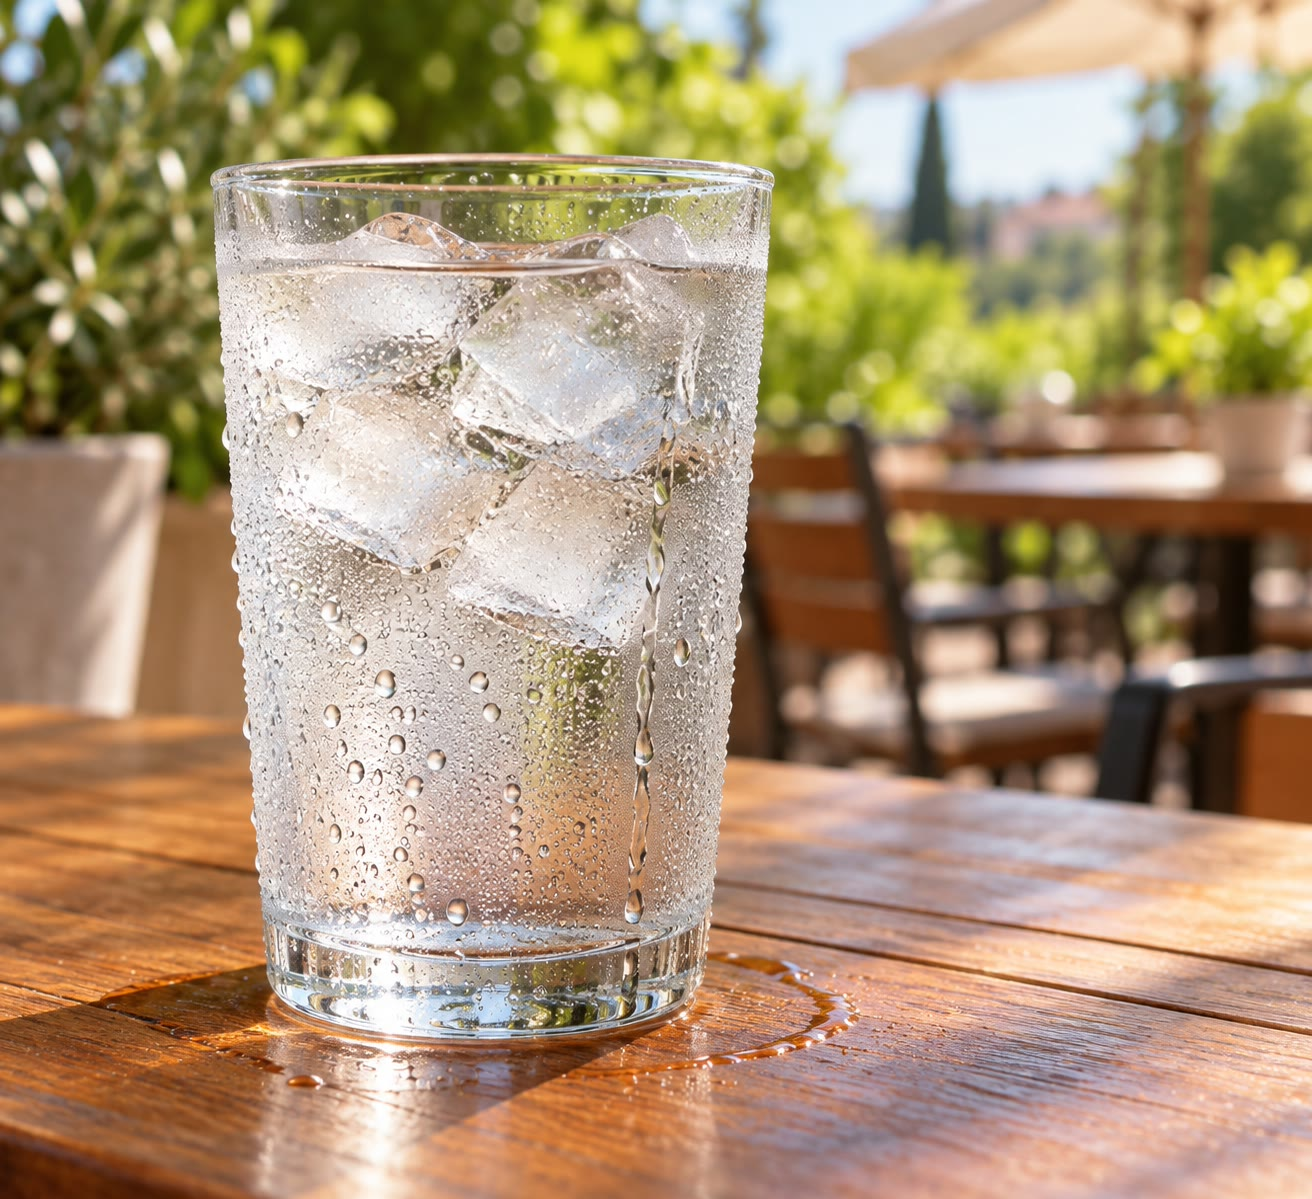
\includegraphics[width=0.5\linewidth]{images/book2/ai/g10-cold-glass.jpg}

{\small Um copo de água gelada num terraço, no verão: gotas se formam do
lado de fora, onde o ar que toca o vidro se resfria.}
\end{omfigure}

\begin{recall}
As nuvens são feitas de minúsculas gotículas de água ou de cristais de
gelo; elas são classificadas em famílias pela forma e pela altura, e dão
chuva, neve e granizo, medidos com um pluviômetro (Livro 1, 4º ano). A
temperatura do ar diminui com a altura na camada mais baixa da atmosfera,
em média cerca de \qty{6.5}{\degreeCelsius} por quilômetro; é o gradiente
térmico vertical do ar ambiente, e as frentes separam massas de ar de
temperaturas diferentes (Livro 1, 8º ano). A pressão diminui com a altura
(os livros de física). A água evapora e se condensa, e a evaporação absorve
um \omterm{def:g10:earth-energy-budget:latent-heat}{calor latente} que a condensação devolve (os livros de física e o
\cref{ch:g10:earth-energy-budget}).
\end{recall}
% ledger: nasa:grc-atmosphere

\section{Vapor de água e saturação}

O ar sempre contém algum vapor de água, um gás invisível. Quanto ele pode
conter depende sobretudo da sua temperatura.

\begin{definition}[Saturação; umidade relativa]\label{def:g10:why-clouds-form:humidity}
O ar está \emph{saturado}\index{saturacao@saturação} quando contém a maior
massa de vapor de água que pode conter à sua temperatura, o seu \emph{teor
de saturação}; todo vapor a mais se condensa em gotículas. A \emph{umidade
relativa}\index{umidade relativa} do ar é o seu teor de vapor de água
dividido pelo seu teor de saturação à mesma temperatura e à mesma pressão,
expresso em porcentagem.
\end{definition}

O teor de água do ar é medido aqui em gramas de vapor por quilograma de ar
seco (\unit{g/kg}): uma parcela de ar que sobe ou desce sem ganhar nem
perder água conserva o mesmo teor, mesmo quando se expande.

\begin{omfigure}
\begin{tikzpicture}
\begin{axis}[omrecord, width=0.88\linewidth, height=6.2cm, xmin=-10, xmax=40,
  ymin=0, ymax=50, xlabel={temperatura (\unit{\degreeCelsius})},
  ylabel={teor de saturação (\unit{g/kg})}, xtick={-10,0,...,40},
  tick label style={font=\small}, label style={font=\small}]
\addplot[omDef!85!black, thick] table[x=T_C, y=ws_gkg] {figdata/out/grade-10-clouds-sat.dat};
\addplot[only marks, mark=*, mark size=1.8pt, omThm!85!black] coordinates {(28,11.37)};
\addplot[only marks, mark=o, mark size=1.8pt, omThm!85!black] coordinates {(16,11.37)};
\draw[->, omThm!85!black, thick] (axis cs:27.2,11.37) -- (axis cs:16.9,11.37);
\node[anchor=north, font=\footnotesize, omThm!85!black] at (axis cs:28,10.6) {ar a \qty{28}{\degreeCelsius}};
\node[anchor=south east, font=\footnotesize, omThm!85!black] at (axis cs:15.5,12.2) {ponto de orvalho};
\node[anchor=south east, font=\footnotesize, omDef!85!black, align=right] at (axis cs:31,34) {acima da curva:\\o vapor se condensa};
\node[anchor=south west, font=\footnotesize, omDef!85!black] at (axis cs:31,2.5) {não saturado};
\node[anchor=north west, font=\footnotesize, omDef!85!black] at (axis cs:34,31.5) {saturação};
\end{axis}
\end{tikzpicture}

{\small A maior massa de vapor de água que um quilograma de ar pode conter,
em função da temperatura, à pressão do nível do mar (sobre água líquida;
calculada com o padrão internacional para a água). O ar a
\qty{28}{\degreeCelsius} com \qty{11.4}{g/kg} (ponto cheio) está longe da
\omterm{def:g10:why-clouds-form:humidity}{saturação}; resfriado sem perder água, ele fica \omterm{def:g10:why-clouds-form:humidity}{saturado} a
\qty{16}{\degreeCelsius} (círculo).}
\end{omfigure}
% ledger: iapws:vapour-pressure, ciaaw:abridged-2024, earth:Mmol, const:R (computed in figdata/grade-10/clouds.py)

A curva sobe abruptamente: \qty{3.8}{g/kg} a \qty{0}{\degreeCelsius},
\qty{14.7}{g/kg} a \qty{20}{\degreeCelsius}, \qty{27.2}{g/kg} a
\qty{30}{\degreeCelsius}. Cada \qty{10}{\degreeCelsius} de aquecimento quase
dobra a água que o ar pode conter. É por isso que o ar tropical pode trazer
chuvas torrenciais, e que o ar de um inverno polar, mesmo \omterm{def:g10:why-clouds-form:humidity}{saturado}, quase
não contém nada.

\begin{definition}[Ponto de orvalho]\label{def:g10:why-clouds-form:dew-point}
O \emph{ponto de orvalho}\index{ponto de orvalho} do ar é a temperatura até
a qual ele precisa ser resfriado, conservando o seu teor de água e a sua
pressão, para ficar \omterm{def:g10:why-clouds-form:humidity}{saturado}.
\end{definition}

\begin{method}[Umidade relativa e ponto de orvalho a partir de uma tabela]\label{met:g10:why-clouds-form:table}
\begin{enumerate}
  \item Leia na tabela o teor de \omterm{def:g10:why-clouds-form:humidity}{saturação} à temperatura do ar.
  \item \omterm{def:g10:why-clouds-form:humidity}{Umidade relativa}: divida por ele o teor de água do ar.
  \item \omterm{def:g10:why-clouds-form:dew-point}{Ponto de orvalho}: encontre na tabela a temperatura cujo teor de
        \omterm{def:g10:why-clouds-form:humidity}{saturação} é igual ao teor de água do ar.
\end{enumerate}
\end{method}

\begin{example}[Uma manhã de verão]\label{ex:g10:why-clouds-form:morning}
% ledger: iapws:vapour-pressure (values computed in figdata/grade-10/clouds.py)
A \qty{20}{\degreeCelsius}, o ar contém \qty{11.4}{g/kg}. O teor de
\omterm{def:g10:why-clouds-form:humidity}{saturação} a \qty{20}{\degreeCelsius} é de \qty{14.7}{g/kg}, logo a \omterm{def:g10:why-clouds-form:humidity}{umidade
relativa} é $11.4/14.7 \approx \qty{78}{\percent}$. O teor de \omterm{def:g10:why-clouds-form:humidity}{saturação} é de
\qty{11.4}{g/kg} a \qty{16}{\degreeCelsius}: esse é o \omterm{def:g10:why-clouds-form:dew-point}{ponto de orvalho}. À
tarde, o mesmo ar aquecido a \qty{28}{\degreeCelsius} (teor de \omterm{def:g10:why-clouds-form:humidity}{saturação}
\qty{24.1}{g/kg}) tem uma \omterm{def:g10:why-clouds-form:humidity}{umidade relativa} de apenas \qty{47}{\percent} ---
com exatamente a mesma água.
\end{example}

O copo da abertura está mais frio que o \omterm{def:g10:why-clouds-form:dew-point}{ponto de orvalho} do ar à sua volta:
o ar que o toca se resfria abaixo do seu \omterm{def:g10:why-clouds-form:dew-point}{ponto de orvalho} e deixa água sobre
o vidro. Numa noite de céu limpo, a grama e o teto dos carros perdem calor
irradiando infravermelho para o céu e ficam mais frios que o ar: forma-se
orvalho sobre eles, ou geada abaixo de \qty{0}{\degreeCelsius}. Quando uma
camada inteira de ar perto do chão se resfria até o seu \omterm{def:g10:why-clouds-form:dew-point}{ponto de orvalho},
gotículas se formam no próprio ar: é a neblina.

\begin{omfigure}
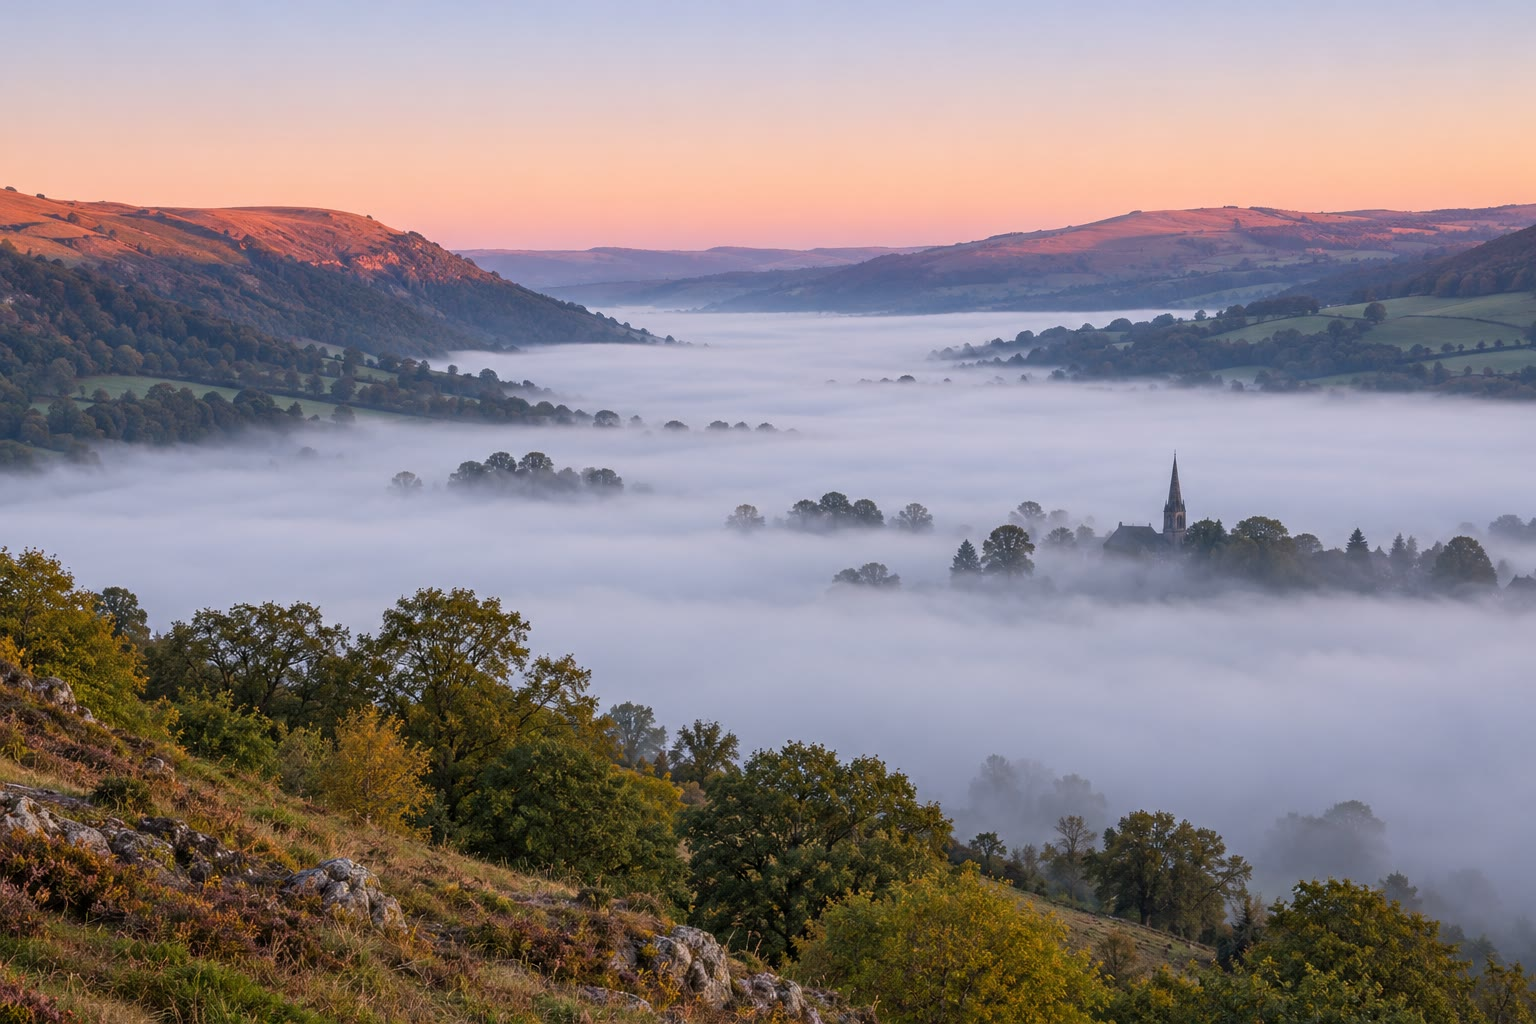
\includegraphics[width=0.75\linewidth]{images/book2/ai/g10-valley-fog.jpg}

{\small Neblina enchendo um vale ao amanhecer. Durante a noite de céu
limpo, o chão se resfriou, o ar frio escorreu para o fundo do vale e ali se
resfriou abaixo do seu \omterm{def:g10:why-clouds-form:dew-point}{ponto de orvalho}.}
\end{omfigure}

\section{O ar que sobe se resfria}

A maioria das nuvens não se forma porque o ar toca algo frio. Elas se formam
porque o ar sobe. A pressão diminui com a altura; uma parcela de ar que sobe
se expande, empurrando o ar em volta, e a energia desse trabalho é retirada
da própria parcela.

\begin{definition}[Resfriamento adiabático; gradiente adiabático seco]\label{def:g10:why-clouds-form:adiabatic}
O \emph{resfriamento adiabático}\index{resfriamento adiabatico@resfriamento adiabático}
é o resfriamento de uma parcela de ar que se expande sem trocar calor com o
que a cerca. A taxa com que o ar não \omterm{def:g10:why-clouds-form:humidity}{saturado} que sobe se resfria dessa
maneira é o
\emph{gradiente adiabático seco}\index{gradiente adiabatico seco@gradiente adiabático seco},
perto de \qty{9.8}{\degreeCelsius} por quilômetro de subida; o ar que desce
se aquece à mesma taxa.
\end{definition}

\begin{proposition}[O gradiente adiabático seco]\label{prop:g10:why-clouds-form:dry-rate}
O \omterm{def:g10:why-clouds-form:adiabatic}{gradiente adiabático seco} é $g/c_p$, em que $g = \qty{9.81}{m/s^2}$ e $c_p
\approx \qty{1005}{J.kg^{-1}.K^{-1}}$ é a energia que aquece um quilograma
de ar em um grau a pressão constante: $9.81/1005 \approx
\qty{0.0098}{\degreeCelsius/m}$, isto é, \qty{9.8}{\degreeCelsius/km}.
(Admitido: a demonstração cabe aos livros de física.)
\end{proposition}
% ledger: const:gn, const:R, earth:Mmol (c_p of dry air computed as (7/2)R/M in figdata/grade-10/clouds.py)

O \omterm{def:g10:why-clouds-form:dew-point}{ponto de orvalho} da parcela também baixa à medida que ela sobe, mas
devagar: o seu teor de água continua o mesmo, enquanto a queda da pressão
torna o vapor um pouco mais fácil de saturar. O cálculo para o ar perto do
chão dá cerca de \qty{1.8}{\degreeCelsius} por quilômetro. A temperatura da
parcela se aproxima, portanto, do seu \omterm{def:g10:why-clouds-form:dew-point}{ponto de orvalho} em cerca de
$9.8 - 1.8 = \qty{8}{\degreeCelsius}$ a cada quilômetro de subida.
% ledger: iapws:vapour-pressure (dew-point rate computed in figdata/grade-10/clouds.py)

\begin{definition}[Nível de condensação]\label{def:g10:why-clouds-form:condensation-level}
O \emph{nível de condensação}\index{nivel de condensacao@nível de condensação}
de uma parcela de ar é a altura em que, ao subir, ela fica \omterm{def:g10:why-clouds-form:humidity}{saturada}. Acima
dele a água se condensa: o nível de condensação é a base plana das nuvens
que o ar ascendente forma.
\end{definition}

\begin{proposition}[Altura do nível de condensação]\label{prop:g10:why-clouds-form:lcl}
O ar que sobe do chão com temperatura $T$ e \omterm{def:g10:why-clouds-form:dew-point}{ponto de orvalho} $T_d$
(em \unit{\degreeCelsius}) fica \omterm{def:g10:why-clouds-form:humidity}{saturado} a cerca de
\[
  z = \frac{T - T_d}{8}\ \text{km} = \qty{125}{m} \times (T - T_d).
\]
\end{proposition}

\begin{proof}
A uma altura $z$ (em km), a temperatura da parcela é $T - 9.8\,z$ e o seu
\omterm{def:g10:why-clouds-form:dew-point}{ponto de orvalho} é $T_d - 1.8\,z$. Ela fica \omterm{def:g10:why-clouds-form:humidity}{saturada} quando os dois são
iguais: $T - 9.8\,z = T_d - 1.8\,z$, logo $8\,z = T - T_d$ e
$z = (T - T_d)/8$ km. Um oitavo de quilômetro são \qty{125}{m}.
\end{proof}

\begin{example}[Um cúmulo à tarde]\label{ex:g10:why-clouds-form:base}
% ledger: iapws:vapour-pressure (exact ascent computed in figdata/grade-10/clouds.py: 1.51 km)
Na tarde do \cref{ex:g10:why-clouds-form:morning}, o ar junto ao chão está
a \qty{28}{\degreeCelsius}, com \omterm{def:g10:why-clouds-form:dew-point}{ponto de orvalho} de \qty{16}{\degreeCelsius}.
As bolhas que sobem ficam \omterm{def:g10:why-clouds-form:humidity}{saturadas} a $125 \times 12 = \qty{1500}{m}$: os
cúmulos têm a base plana a cerca de \qty{1.5}{km} de altura. De manhã, a
\qty{20}{\degreeCelsius}, o mesmo ar teria se condensado a apenas
$125 \times 4 = \qty{500}{m}$: a base das nuvens sobe ao longo do dia, à
medida que o chão se aquece.
\end{example}

\section{Ar estável e ar instável}

Se uma parcela que sobe continua subindo depende do ar à sua volta. Uma
parcela mais quente que o que a cerca é mais leve que o ar que ela desloca
e sobe, como um balão de ar quente; uma parcela mais fria que o que a cerca
volta a descer.

\begin{definition}[Ar estável; ar instável]\label{def:g10:why-clouds-form:stability}
O ar é \emph{estável}\index{ar estavel@ar estável} quando uma parcela
empurrada para cima fica mais fria que o ar à sua volta e, por isso, volta a
descer até o ponto de partida. Ele é \emph{instável}\index{ar instavel@ar instável}
quando a parcela fica mais quente que o ar à sua volta e continua subindo
sozinha.
\end{definition}

A parcela que sobe se resfria segundo o \omterm{def:g10:why-clouds-form:adiabatic}{gradiente adiabático seco},
\qty{9.8}{\degreeCelsius} por quilômetro, enquanto não está \omterm{def:g10:why-clouds-form:humidity}{saturada}. Uma vez
\omterm{def:g10:why-clouds-form:humidity}{saturada}, ela se resfria mais devagar: a condensação libera \omterm{def:g10:earth-energy-budget:latent-heat}{calor latente}
dentro da parcela. O cálculo dá cerca de \qty{4.7}{\degreeCelsius} por
quilômetro no ar quente perto do chão, cerca de \num{5.8} a
\qty{0}{\degreeCelsius}, e mais no ar frio mais alto, onde resta pouca água
para condensar; é o gradiente adiabático \omterm{def:g10:why-clouds-form:humidity}{saturado}. (A sua fórmula é
deduzida nos volumes universitários.)
% ledger: nist:water-latent, iapws:vapour-pressure (saturated rates computed in figdata/grade-10/clouds.py)

\begin{method}[Este ar é estável?]\label{met:g10:why-clouds-form:stable}
\begin{enumerate}
  \item Descubra com que rapidez a temperatura do ar em volta diminui com a
        altura (o gradiente térmico vertical do ar ambiente, dado por uma
        sondagem com balão).
  \item Compare-a com a taxa com que a parcela se resfria: o gradiente
        seco, cerca de \qty{9.8}{\degreeCelsius/km}, abaixo do seu \omterm{def:g10:why-clouds-form:condensation-level}{nível de
        condensação}; o gradiente \omterm{def:g10:why-clouds-form:humidity}{saturado}, cerca de
        \qty{5}{\degreeCelsius/km}, acima dele.
  \item Se o ar em volta se resfria mais devagar que a parcela, a parcela
        acaba mais fria: \omterm{def:g10:why-clouds-form:stability}{estável}. Se ele se resfria mais depressa, a parcela
        acaba mais quente: \omterm{def:g10:why-clouds-form:stability}{instável}. Uma camada em que a temperatura
        \emph{aumenta} com a altura é muito \omterm{def:g10:why-clouds-form:stability}{estável}: ela detém o ar que
        sobe como uma tampa.
\end{enumerate}
\end{method}

Com o gradiente médio de cerca de \qty{6.5}{\degreeCelsius/km}, o ar é
\omterm{def:g10:why-clouds-form:stability}{estável} enquanto não está \omterm{def:g10:why-clouds-form:humidity}{saturado} (a parcela se resfria mais depressa) e
\omterm{def:g10:why-clouds-form:stability}{instável} quando está \omterm{def:g10:why-clouds-form:humidity}{saturado} (a parcela se resfria mais devagar). Diz-se
que esse ar é condicionalmente \omterm{def:g10:why-clouds-form:stability}{instável}: ele é \omterm{def:g10:why-clouds-form:stability}{estável}, a não ser que algo o
levante até o seu \omterm{def:g10:why-clouds-form:condensation-level}{nível de condensação}, e então a nuvem cresce por si só.

\begin{omfigure}
\begin{tikzpicture}
\begin{axis}[omrecord, width=0.9\linewidth, height=7.6cm, xmin=-30, xmax=36,
  ymin=0, ymax=6, xlabel={temperatura (\unit{\degreeCelsius})}, ylabel={altura (km)},
  xtick={-30,-20,...,30}, ytick={0,1,...,6},
  legend style={at={(0.02,0.98)}, anchor=north west, font=\footnotesize, draw=black!30, fill=white},
  tick label style={font=\small}, label style={font=\small}]
\fill[omDef!10] (axis cs:-30,1.51) rectangle (axis cs:36,3.96);
\addplot[black!60, thick] table[x=T_C, y=z_km] {figdata/out/grade-10-clouds-envA.dat};
\addlegendentry{sondagem A}
\addplot[omProp!90!black, thick, densely dotted] table[x=T_C, y=z_km] {figdata/out/grade-10-clouds-envB.dat};
\addlegendentry{sondagem B}
\addplot[omThm!85!black, very thick] table[x=T_C, y=z_km] {figdata/out/grade-10-clouds-parcel.dat};
\addlegendentry{parcela que sobe}
\addplot[omMeth!85!black, thick, dashed] table[x=Td_C, y=z_km] {figdata/out/grade-10-clouds-dew.dat};
\addlegendentry{o seu ponto de orvalho}
\draw[black!50, dashed] (axis cs:-30,1.51) -- (axis cs:36,1.51);
\node[anchor=south west, font=\footnotesize] at (axis cs:-29.5,1.53) {nível de condensação};
\node[anchor=north east, font=\footnotesize, omDef!80!black] at (axis cs:35.5,3.9) {nuvem com A};
\end{axis}
\end{tikzpicture}

{\small Uma parcela que sobe do chão a \qty{28}{\degreeCelsius} com \omterm{def:g10:why-clouds-form:dew-point}{ponto de
orvalho} de \qty{16}{\degreeCelsius} (calculada): ela se resfria segundo o
gradiente seco até que a sua temperatura encontre o seu \omterm{def:g10:why-clouds-form:dew-point}{ponto de orvalho}, a
\qty{1.5}{km}, e depois segundo o gradiente \omterm{def:g10:why-clouds-form:humidity}{saturado}, mais lento. Duas
sondagens inventadas: em A, a parcela é mais quente que o ar em volta desde
\qty{1.5}{km} até a camada quente perto de \qty{4}{km}, e um cúmulo cresce
entre as duas (sombreado); em B, um ar mais quente acima do chão mantém a
parcela mais fria que o ar em volta em toda parte: \omterm{def:g10:why-clouds-form:stability}{ar estável}, nenhum
cúmulo.}
\end{omfigure}
% ledger: iapws:vapour-pressure, nist:water-latent (parcel computed in figdata/grade-10/clouds.py; soundings invented)

Quando o ar é \omterm{def:g10:why-clouds-form:stability}{estável} e é levantado mesmo assim --- sobre uma montanha, ou
ao longo de uma frente ---, as nuvens que se formam se espalham em camadas
cinzentas e planas: os estratos. Quando ele é \omterm{def:g10:why-clouds-form:stability}{instável}, as nuvens se
avolumam para cima em montes: os cúmulos e, quando a instabilidade chega
alto o bastante, os cumulonimbos das trovoadas, cujo topo se espalha numa
bigorna quando encontra o ar muito \omterm{def:g10:why-clouds-form:stability}{estável} acima da camada mais baixa da
atmosfera.

\begin{omfigure}
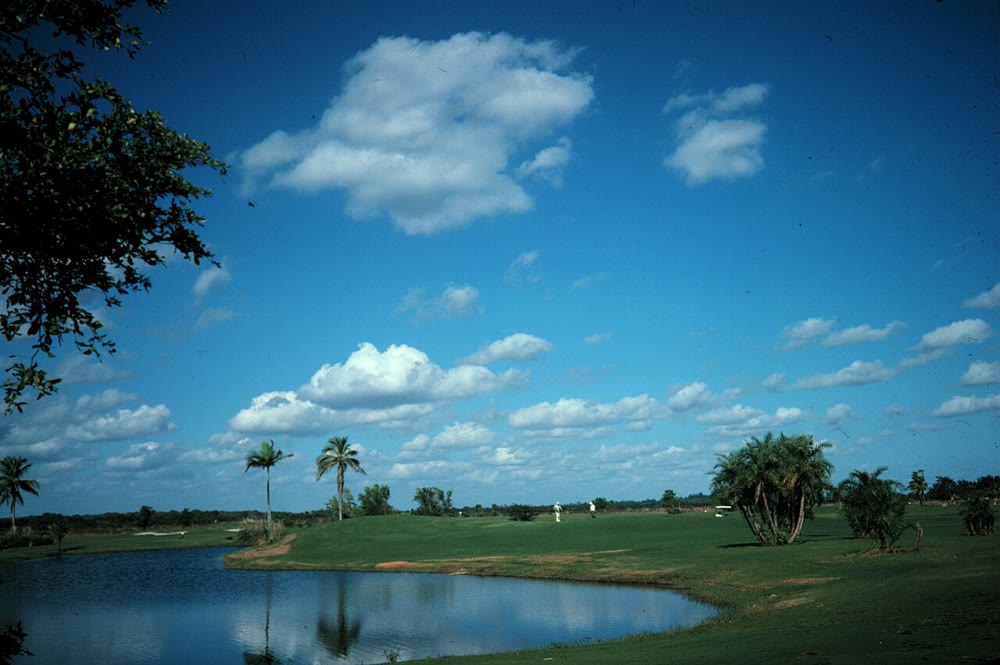
\includegraphics[height=4.5cm]{images/book2/g10-noaa-fair-weather-cumulus.jpg}\hspace{0.6em}%
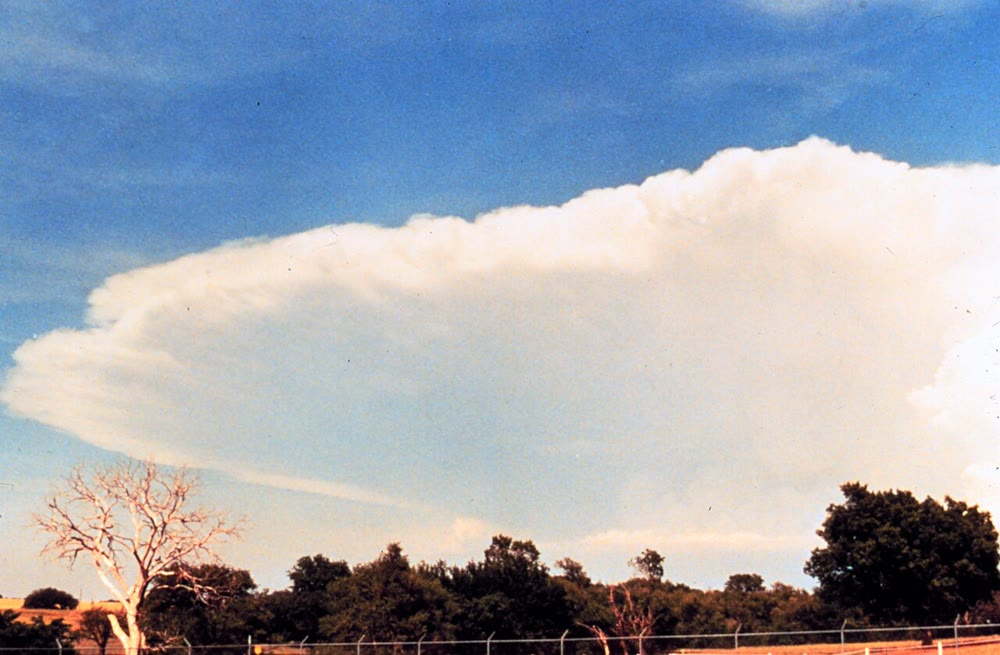
\includegraphics[height=4.5cm]{images/book2/g10-noaa-cumulonimbus-anvil.jpg}

{\small À esquerda: cúmulos de bom tempo sobre a Flórida, com a base plana
no seu \omterm{def:g10:why-clouds-form:condensation-level}{nível de condensação}. Fotografia: Ralph F. Kresge, NOAA (domínio
público). À direita: a bigorna de um cumulonimbo nas primeiras fases de uma
tempestade. Fotografia: NOAA National Severe Storms Laboratory (domínio
público).}
\end{omfigure}

\section{Quatro maneiras de levantar o ar}

O ar sobe por quatro razões.
\begin{itemize}
  \item \textbf{Aquecimento por baixo.} Num dia de sol, o chão aquece o ar
        acima dele; bolhas de ar quente sobem das manchas mais quentes. São
        elas que dão os cúmulos da tarde.
  \item \textbf{Montanhas.} O vento que sopra contra uma cordilheira é
        forçado a subir pela sua encosta.
  \item \textbf{Frentes.} Onde massas de ar quente e de ar frio se
        encontram, o ar quente, mais leve, sobe por cima do ar frio, ou o ar
        frio se enfia por baixo dele (Livro 1, 8º ano).
  \item \textbf{Convergência.} Quando os ventos convergem perto do chão, o
        ar não tem para onde ir a não ser para cima, como na faixa de ar
        ascendente perto do equador e no centro de uma depressão.
\end{itemize}

\begin{method}[Seguir uma parcela sobre uma montanha]\label{met:g10:why-clouds-form:mountain}
\begin{enumerate}
  \item Encontre o \omterm{def:g10:why-clouds-form:condensation-level}{nível de condensação} com a regra dos 125 metros; até ele,
        a parcela se resfria a \qty{9.8}{\degreeCelsius/km}.
  \item Dali até a crista, ela se resfria segundo o gradiente \omterm{def:g10:why-clouds-form:humidity}{saturado}; a
        água que se condensa cai como chuva ou neve na encosta de
        barlavento.
  \item Depois da crista, a parcela desce, não \omterm{def:g10:why-clouds-form:humidity}{saturada}: ela se aquece a
        \qty{9.8}{\degreeCelsius/km} durante toda a descida.
\end{enumerate}
\end{method}

\begin{example}[O vento quente e seco de sotavento]\label{ex:g10:why-clouds-form:lee}
% ledger: iapws:vapour-pressure, nist:water-latent (all values computed in figdata/grade-10/clouds.py)
Um ar ao nível do mar a \qty{20}{\degreeCelsius}, com \omterm{def:g10:why-clouds-form:dew-point}{ponto de orvalho} de
\qty{12}{\degreeCelsius}, é empurrado sobre uma serra de \qty{2500}{m} de
altura. Ele fica \omterm{def:g10:why-clouds-form:humidity}{saturado} a $125 \times 8 = \qty{1000}{m}$, a cerca de
\qty{10}{\degreeCelsius}. Dali até a crista, ele se resfria segundo o
gradiente \omterm{def:g10:why-clouds-form:humidity}{saturado}, até cerca de \qty{2}{\degreeCelsius}, e perde como chuva
cerca de um terço da sua água (de \num{8.7} para \qty{6.0}{g/kg}). Descendo
pelo outro lado, ele se aquece segundo o gradiente seco ao longo de
\qty{2.5}{km}: chega à planície a cerca de \qty{27}{\degreeCelsius}, sete
graus mais quente do que no início, com uma \omterm{def:g10:why-clouds-form:humidity}{umidade relativa} de cerca de
\qty{27}{\percent}. Ventos quentes e secos como esse sopram a sotavento de
muitas cordilheiras.
\end{example}

\begin{omfigure}
\begin{tikzpicture}[font=\footnotesize, >={Stealth[length=2mm]}]
  \fill[omExo!30] (0,0) -- (3.5,0.3) -- (6,3.0) -- (8.5,0.3) -- (12,0) -- (12,-0.25) -- (0,-0.25) -- cycle;
  \draw[thick, black!70] (0,0) -- (3.5,0.3) -- (6,3.0) -- (8.5,0.3) -- (12,0);
  \draw[black!40, dashed] (0,1.2) -- (4.6,1.2);
  \node[anchor=south west, black!60, align=left] at (0.1,1.22) {nível de\\condensação, \qty{1000}{m}};
  \foreach \x in {3.62,3.86,4.1} \draw[omDef!60] (\x,1.2) -- (\x-0.06,{0.3+(\x-0.06-3.5)*1.08+0.04});
  \pic[scale=1.1, transform shape] at (4.6,1.22) {puffycloud};
  \pic[scale=0.9, transform shape] at (5.0,2.2) {puffycloud};
  \draw[->, thick, omDef!80!black] (0.2,0.25) -- (2.8,0.5) .. controls (3.6,0.75) .. (4.4,1.7) -- (5.4,2.9) .. controls (5.8,3.4) and (6.2,3.4) .. (6.6,2.9) -- (7.6,1.7) .. controls (8.4,0.75) .. (9.2,0.5) -- (11.8,0.25);
  \node[anchor=east, align=right] at (3.4,2.15) {\qty{10}{\degreeCelsius}, saturado};
  \node[anchor=south, align=center] at (6.0,3.45) {crista a \qty{2500}{m}: \qty{2}{\degreeCelsius}};
  \node[anchor=west, align=left] at (7.75,2.1) {desce e se aquece\\a \qty{9.8}{\degreeCelsius/km}};
  \node[anchor=north, align=center] at (1.0,-0.3) {\qty{20}{\degreeCelsius}\\ponto de orvalho \qty{12}{\degreeCelsius}};
  \node[anchor=north, align=center] at (11.0,-0.3) {\qty{27}{\degreeCelsius}\\ponto de orvalho \qty{6}{\degreeCelsius}};
  \node[anchor=north, black!60] at (4.0,-0.3) {barlavento: chuva};
  \node[anchor=north, black!60] at (8.2,-0.3) {sotavento: seco};
\end{tikzpicture}

{\small Uma parcela de ar atravessando uma serra (temperaturas calculadas;
escala vertical exagerada). Ela se resfria segundo o gradiente seco até o
seu \omterm{def:g10:why-clouds-form:condensation-level}{nível de condensação}, segundo o gradiente \omterm{def:g10:why-clouds-form:humidity}{saturado}, mais lento, acima
dele, perdendo água como chuva, e se aquece segundo o gradiente seco
durante toda a descida pela encosta de sotavento.}
\end{omfigure}

\section{Das gotículas à chuva e à neve}

O vapor de água não se condensa facilmente num ar perfeitamente limpo. As
gotículas se formam sobre partículas de matéria.

\begin{definition}[Núcleo de condensação]\label{def:g10:why-clouds-form:nucleus}
Um \emph{núcleo de condensação}\index{nucleo de condensacao@núcleo de condensação}
é uma partícula minúscula em suspensão no ar --- um grão de sal marinho,
poeira, fumaça ou fuligem --- sobre a qual o vapor de água se condensa para
formar uma gotícula de nuvem.
\end{definition}

Um núcleo típico mede cerca de \qty{0.0002}{mm}, uma gotícula de nuvem
cerca de \qty{0.02}{mm}, uma gota de garoa \qty{0.5}{mm} e uma gota de chuva
cerca de \qty{2}{mm}. Uma gota de chuva é cem vezes mais larga que uma
gotícula de nuvem, logo o seu volume é $100^3$ vezes maior: um milhão de
gotículas de nuvem formam uma gota de chuva. As gotículas de nuvem são tão
pequenas que a menor corrente ascendente as mantém no ar; para que a chuva
caia, as gotículas precisam crescer cem vezes.
% ledger: jpl:drop-sizes

\begin{omfigure}
\begin{tikzpicture}
\begin{axis}[width=0.9\linewidth, height=3.4cm, xmode=log, xmin=1e-4, xmax=10,
  ymin=0, ymax=1, axis y line=none, axis x line*=bottom,
  xlabel={diâmetro (mm), escala logarítmica}, tick label style={font=\small},
  label style={font=\small}, clip=false]
\addplot[only marks, mark=*, omDef!85!black, mark size=2.5pt] coordinates {(0.0002,0.3) (0.02,0.3) (0.5,0.3) (2,0.3)};
\node[anchor=south, font=\footnotesize, align=center] at (axis cs:0.0002,0.42) {núcleo de\\condensação};
\node[anchor=south, font=\footnotesize, align=center] at (axis cs:0.02,0.42) {gotícula\\de nuvem};
\node[anchor=south, font=\footnotesize, align=center] at (axis cs:0.5,0.42) {garoa};
\node[anchor=south, font=\footnotesize, align=center] at (axis cs:2,0.42) {gota de chuva};
\end{axis}
\end{tikzpicture}

{\small Tamanhos típicos, numa escala em que cada passo vale dez vezes o
anterior: cada objeto é cerca de cem vezes mais largo que o anterior, com
exceção da garoa. Dados: NASA Jet Propulsion Laboratory.}
\end{omfigure}

Dois processos as fazem crescer.

\begin{definition}[Processo da chuva quente; processo dos cristais de gelo]\label{def:g10:why-clouds-form:rain-processes}
No \emph{processo da chuva quente}\index{processo da chuva quente}, as
gotículas maiores de uma nuvem caem mais depressa que as pequenas, chocam-se
com elas e se fundem, crescendo enquanto caem. No
\emph{processo dos cristais de gelo}\index{processo dos cristais de gelo},
na parte de uma nuvem mais fria que \qty{0}{\degreeCelsius}, onde cristais
de gelo e gotículas super-resfriadas (líquidas abaixo de
\qty{0}{\degreeCelsius}) estão misturados, os cristais crescem tomando o
vapor que as gotículas evaporam; eles caem como flocos de neve e derretem
em gotas de chuva se o ar abaixo for quente.
\end{definition}

O \omterm{def:g10:why-clouds-form:rain-processes}{processo dos cristais de gelo} funciona porque o teor de \omterm{def:g10:why-clouds-form:humidity}{saturação} é menor
sobre o gelo do que sobre a água líquida à mesma temperatura: a
\qty{-10}{\degreeCelsius}, a pressão de vapor de \omterm{def:g10:why-clouds-form:humidity}{saturação} é de
\qty{287}{Pa} sobre a água e de \qty{260}{Pa} sobre o gelo. Um ar \omterm{def:g10:why-clouds-form:humidity}{saturado}
para as gotículas contém \qty{10}{\percent} de vapor a mais do que o gelo
suporta: o vapor se condensa sobre os cristais, e as gotículas evaporam
para repô-lo.
% ledger: iapws:vapour-pressure, iapws:melt-subl (computed in figdata/grade-10/clouds.py)

\begin{remark}[O calor latente alimenta a tempestade]\label{rem:g10:why-clouds-form:latent}
Cada quilograma de água que se condensa numa nuvem dá ao ar cerca de
\qty{2.5}{MJ}, o \omterm{def:g10:earth-energy-budget:latent-heat}{calor latente} retirado do mar ou do chão quando ela
evaporou (\cref{ch:g10:earth-energy-budget}). É esse calor que torna o
gradiente \omterm{def:g10:why-clouds-form:humidity}{saturado} mais lento que o gradiente seco e mantém um cumulonimbo
subindo; o \cref{ch:g10:storms-and-cyclones} o acompanha até as maiores
tempestades.
\end{remark}
% ledger: nist:water-latent

\section{Exercícios}

Nestes exercícios, use os teores de \omterm{def:g10:why-clouds-form:humidity}{saturação} (em \unit{g/kg}, à pressão do
nível do mar) da tabela abaixo, o gradiente seco
\qty{9.8}{\degreeCelsius/km}, uma queda do \omterm{def:g10:why-clouds-form:dew-point}{ponto de orvalho} de
\qty{1.8}{\degreeCelsius/km} e um gradiente \omterm{def:g10:why-clouds-form:humidity}{saturado} de
\qty{5}{\degreeCelsius/km}.
% ledger: iapws:vapour-pressure (table from figdata/out/grade-10-clouds-sat.dat, rounded)

\begin{center}
\small
\begin{tabular}{l*{11}{c}}
\hline
temperatura (\unit{\degreeCelsius}) & 0 & 4 & 8 & 10 & 12 & 14 & 16 & 20 & 24 & 28 & 30 \\
teor de \omterm{def:g10:why-clouds-form:humidity}{saturação} (\unit{g/kg}) & 3.8 & 5.0 & 6.7 & 7.6 & 8.7 & 10.0 & 11.4 & 14.7 & 18.9 & 24.1 & 27.2 \\
\hline
\end{tabular}
\end{center}

\begin{exercise}[$\star$]\label{exo:g10:why-clouds-form:1}
Defina a \omterm{def:g10:why-clouds-form:humidity}{umidade relativa} e o \omterm{def:g10:why-clouds-form:dew-point}{ponto de orvalho} do ar.
\end{exercise}

\begin{exercise}[$\star$]\label{exo:g10:why-clouds-form:2}
A partir da tabela, dê o teor de \omterm{def:g10:why-clouds-form:humidity}{saturação} a \num{0}, \num{10}, \num{20} e
\qty{30}{\degreeCelsius}. Por aproximadamente que fator ele cresce a cada
\qty{10}{\degreeCelsius} de aquecimento?
\end{exercise}

\begin{exercise}[$\star$]\label{exo:g10:why-clouds-form:3}
Um ar a \qty{24}{\degreeCelsius} contém \qty{10.0}{g/kg} de vapor de água.
Encontre a sua \omterm{def:g10:why-clouds-form:humidity}{umidade relativa} e o seu \omterm{def:g10:why-clouds-form:dew-point}{ponto de orvalho}.
\end{exercise}

\begin{exercise}[$\star$]\label{exo:g10:why-clouds-form:4}
Explique por que um copo de água gelada ``sua'' no verão, e por que isso não
acontece num dia de inverno muito seco dentro de casa.
\end{exercise}

\begin{exercise}[$\star$]\label{exo:g10:why-clouds-form:5}
Cite as quatro maneiras pelas quais o ar é obrigado a subir, com um exemplo
de cada.
\end{exercise}

\begin{exercise}[$\star\star$]\label{exo:g10:why-clouds-form:6}
Usando a \cref{prop:g10:why-clouds-form:lcl}, encontre a altura da base das
nuvens para um ar a \qty{30}{\degreeCelsius} com \omterm{def:g10:why-clouds-form:dew-point}{ponto de orvalho} de
\qty{18}{\degreeCelsius}, e para um ar a \qty{22}{\degreeCelsius} com \omterm{def:g10:why-clouds-form:dew-point}{ponto
de orvalho} de \qty{20}{\degreeCelsius}. Qual dos dois dias deve ser cinzento
e de nuvens baixas?
\end{exercise}

\begin{exercise}[$\star\star$]\label{exo:g10:why-clouds-form:7}
Uma parcela de ar não \omterm{def:g10:why-clouds-form:humidity}{saturado} sai do chão a \qty{18}{\degreeCelsius}. Qual é
a sua temperatura a \qty{1}{km} e a \qty{2}{km} de altura, se ela continuar
não \omterm{def:g10:why-clouds-form:humidity}{saturada}? Descendo de novo a partir de \qty{2}{km}, a que temperatura
ela chega ao chão?
\end{exercise}

\begin{exercise}[$\star\star$]\label{exo:g10:why-clouds-form:8}
Uma sondagem com balão mostra a temperatura diminuindo
\qty{4}{\degreeCelsius} por km. O ar é \omterm{def:g10:why-clouds-form:stability}{estável} para uma parcela não
\omterm{def:g10:why-clouds-form:humidity}{saturada}? E para uma \omterm{def:g10:why-clouds-form:humidity}{saturada}? Numa tarde quente, a temperatura cai
\qty{12}{\degreeCelsius} no primeiro quilômetro acima do chão: o que
acontece com as bolhas de ar quente?
\end{exercise}

\begin{exercise}[$\star\star$]\label{exo:g10:why-clouds-form:9}
Um ar \omterm{def:g10:why-clouds-form:humidity}{saturado} a \qty{20}{\degreeCelsius} é resfriado até
\qty{10}{\degreeCelsius}. Quantos gramas de água se condensam por quilograma
de ar? Para onde vai o \omterm{def:g10:earth-energy-budget:latent-heat}{calor latente} liberado?
\end{exercise}

\begin{exercise}[$\star\star$]\label{exo:g10:why-clouds-form:10}
Quantas gotículas de nuvem de \qty{0.02}{mm} de diâmetro formam uma gota de
garoa de \qty{0.5}{mm} de diâmetro? E uma gota de chuva de \qty{2}{mm}?
\end{exercise}

\begin{exercise}[$\star\star$]\label{exo:g10:why-clouds-form:11}
Explique, passo a passo, por que a neblina se forma nos vales, e não no alto
dos morros, ao amanhecer, depois de uma noite limpa e calma.
\end{exercise}

\begin{exercise}[$\star\star\star$]\label{exo:g10:why-clouds-form:12}
O gradiente seco é $a$ e o \omterm{def:g10:why-clouds-form:dew-point}{ponto de orvalho} baixa à taxa $b$ (os dois em
\unit{\degreeCelsius/km}). Mostre que o \omterm{def:g10:why-clouds-form:condensation-level}{nível de condensação} fica em
$z = (T - T_d)/(a - b)$. Sobre um planalto elevado, o \omterm{def:g10:why-clouds-form:dew-point}{ponto de orvalho}
baixa \qty{1.7}{\degreeCelsius/km}: em que se transforma a regra
``\qty{125}{m} por grau''?
\end{exercise}

\begin{exercise}[$\star\star\star$]\label{exo:g10:why-clouds-form:13}
Um ar ao nível do mar a \qty{15}{\degreeCelsius}, com \omterm{def:g10:why-clouds-form:dew-point}{ponto de orvalho} de
\qty{11}{\degreeCelsius}, atravessa uma serra de \qty{2000}{m} de altura.
Seguindo o \cref{met:g10:why-clouds-form:mountain}, encontre o \omterm{def:g10:why-clouds-form:condensation-level}{nível de
condensação}, a temperatura ali, a temperatura na crista e a temperatura com
que o ar chega à planície do outro lado.
\end{exercise}

\begin{exercise}[$\star\star\star$]\label{exo:g10:why-clouds-form:14}
A \qty{-20}{\degreeCelsius}, a pressão de vapor de \omterm{def:g10:why-clouds-form:humidity}{saturação} é de
\qty{126}{Pa} sobre a água e de \qty{103}{Pa} sobre o gelo. Em que
porcentagem um ar \omterm{def:g10:why-clouds-form:humidity}{saturado} para as gotículas está supersaturado para o
gelo? Compare com \qty{-10}{\degreeCelsius} e diga em que parte de uma
nuvem o \omterm{def:g10:why-clouds-form:rain-processes}{processo dos cristais de gelo} funciona melhor.
\end{exercise}

\begin{exercise}[$\star\star\star$]\label{exo:g10:why-clouds-form:15}
O ar em volta se resfria \qty{6.5}{\degreeCelsius/km}. Uma parcela parte à
mesma temperatura que o ar em volta e sobe \qty{1}{km}. Calcule a diferença
entre a sua temperatura e a do ar em volta se ela não estiver \omterm{def:g10:why-clouds-form:humidity}{saturada} e,
depois, se estiver \omterm{def:g10:why-clouds-form:humidity}{saturada}. Explique a expressão ``condicionalmente
\omterm{def:g10:why-clouds-form:stability}{instável}''.
\end{exercise}

\section{Problema: uma tarde de verão sobre a planície}

\begin{problem}[{Problema de fim de semana --- da umidade da manhã à base
das nuvens da tarde}]
\label{pb:g10:why-clouds-form:1}
% ledger: iapws:vapour-pressure, nist:water-latent (all results computed in figdata/grade-10/clouds.py or from the rounded data below; the sounding is sounding A, invented)
Sobre uma vasta planície, num dia de verão, o ar perto do chão contém
\qty{11.4}{g/kg} de vapor de água o dia inteiro. Ele está a
\qty{20}{\degreeCelsius} de manhã e a \qty{28}{\degreeCelsius} à tarde. Uma
sondagem com balão (um exemplo inventado) dá a temperatura do ar acima:

\begin{center}
\small
\begin{tabular}{l*{8}{c}}
\hline
altura (km) & 0 & 0.5 & 1.0 & 1.5 & 2.5 & 3.5 & 3.6 & 4.0 \\
temperatura (\unit{\degreeCelsius}) & 28.0 & 23.1 & 18.2 & 13.4 & 6.9 & 0.4 & $-0.3$ & 1.2 \\
\hline
\end{tabular}
\end{center}

\noindent Use a tabela dos teores de \omterm{def:g10:why-clouds-form:humidity}{saturação} e os gradientes dados antes
dos exercícios.

\medskip
\noindent\textbf{Parte I --- A umidade.}
\begin{enumerate}
  \item Dê o teor de \omterm{def:g10:why-clouds-form:humidity}{saturação} a \qty{20}{\degreeCelsius}.
  \item Calcule a \omterm{def:g10:why-clouds-form:humidity}{umidade relativa} da manhã.
  \item Encontre o \omterm{def:g10:why-clouds-form:dew-point}{ponto de orvalho} do ar.
  \item Calcule a \omterm{def:g10:why-clouds-form:humidity}{umidade relativa} à tarde.
  \item O ar ficou mais seco à tarde? Explique.
\end{enumerate}

\medskip
\noindent\textbf{Parte II --- A noite e o orvalho.}
\begin{enumerate}[resume]
  \item Durante a noite, o ar perto do chão se resfria. A que temperatura o
        orvalho começa a se formar?
  \item Se o ar se resfriar até \qty{12}{\degreeCelsius}, quantos gramas de
        água por quilograma de ar terão se condensado?
  \item Por que o orvalho se forma sobre a grama e sobre o teto dos carros
        antes de se formar no ar?
\end{enumerate}

\medskip
\noindent\textbf{Parte III --- A sondagem.}
\begin{enumerate}[resume]
  \item Calcule a taxa com que a temperatura diminui entre \num{0} e
        \qty{1.5}{km}. Compare-a com o gradiente seco.
  \item Calcule-a entre \num{1.5} e \qty{3.5}{km}.
  \item O ar entre \num{1.5} e \qty{3.5}{km} é \omterm{def:g10:why-clouds-form:stability}{estável} para uma parcela não
        \omterm{def:g10:why-clouds-form:humidity}{saturada}? E para uma \omterm{def:g10:why-clouds-form:humidity}{saturada}?
  \item O que acontece entre \num{3.6} e \qty{4.0}{km}? O que isso faz com
        uma nuvem que cresce para cima?
\end{enumerate}

\medskip
\noindent\textbf{Parte IV --- A base das nuvens.}
\begin{enumerate}[resume]
  \item Calcule a diferença entre a temperatura do ar e o seu \omterm{def:g10:why-clouds-form:dew-point}{ponto de
        orvalho} junto ao chão, à tarde.
  \item Calcule a temperatura e o \omterm{def:g10:why-clouds-form:dew-point}{ponto de orvalho} de uma bolha desse ar
        depois de subir \qty{1}{km}, ainda não \omterm{def:g10:why-clouds-form:humidity}{saturada}.
  \item Quanto diminuiu a diferença entre os dois? A que taxa ela diminui?
  \item Mostre que essa taxa dá a regra ``\qty{125}{m} por grau''.
  \item Qual teria sido a base das nuvens de manhã?
  \item Explique por que a base dos cúmulos sobe ao longo do dia.
  \item Escreva a equação que diz que a temperatura da bolha é igual ao seu
        \omterm{def:g10:why-clouds-form:dew-point}{ponto de orvalho} na altura $z$ (em km).
  \item Resolva-a: a que altura fica a base dos cúmulos da tarde?
\end{enumerate}
\end{problem}
